\newpage\EMPHASIZE{16. Scope}

\textsc{Objectives}

\begin{itemize}
\item
  Understand the scope of a variable
\item
  Understand how C++ searches for a variable
\item
  Understand the importance of using minimal scopes
\end{itemize}

I' ve already mentioned scopes of variables in several
places. In this set of notes, I will collect what you already know about
scopes. So much of it is review. I will also add a few new scope rules.

\newpage\EMPHASIZE{Scope}

A variable has a name, a value, and you should know by now, a variable also has a \EMPHASIZE{scope}. This refers to the place in your code where you can refer to that variable.

Here's an old example (very very very old ...):

\begin{console}
x = 42; // x not declared yet bozo!!!

int x = 0;
std::cout << x << std::endl;
\end{console}

In general the scope of a variable is from the \EMPHASIZE{point of declaration} to the \EMPHASIZE{end of the block where it is declared}. During the execution of the program, when the point of execution exits that block, the variable is destroyed. Try this:

\begin{consolethree}[escapeinside=||]
#include <iostream>

int main()
{   
    int x = 0;
    std::cin >> x;

    if (x == 42)
    {   
       |\tikzmarknode{yboxtl}{}|std::cout << "here we go ..." << std::endl;   |\tikzmarknode{yboxtr}{}|
        int y = x + 1;
        std::cout << "y: " << y << std::endl;        |\tikzmarknode{yboxend}{}|
    }  |\tikzmarknode{yboxbl}{}|                                              |\tikzmarknode{yboxbr}{}||\sidebox{scopeybox}{Scope of y}|
    std::cout << "x: " << x << std::endl;

    return 0;
\end{consolethree}
\DrawArrowPoints[dashed,red,thick]{yboxtr}{yboxend}{-- (yboxtl) -- (yboxbl) -- (yboxbr) -- (yboxtr) -- ++(0,-0.9) -- (scopeybox)}

Of course you should know by now that this won't work (try it):

\begin{consolethree}[escapeinside=||]
#include <iostream>

int main()
{    
     int x = 0;
     std::cin >> x;
     
     if (x == 42)
     {    
          std::cout << "here we go ..." << std::endl;
          int y = x + 1;
          std::cout << "y: " << y << std::endl;
     }
     |\tikzmarknode{badynode}{std::cout << "y: " << y << std::endl;}||\sidebox{badtxbox}{BAD!!!}|

     return 0;
} 
\end{consolethree}
\DrawArrow{badtxbox}{badynode}
\newpage %to keep sideboxes and consoles together on the same page
You should visualize the variables in your code as being created in blocks of memory spaces. Suppose the user enters 42 for \texttt{x} and we are about to execute the print statement in the body of the \texttt{if} statement. The memory looks like this:
\sidenote
{
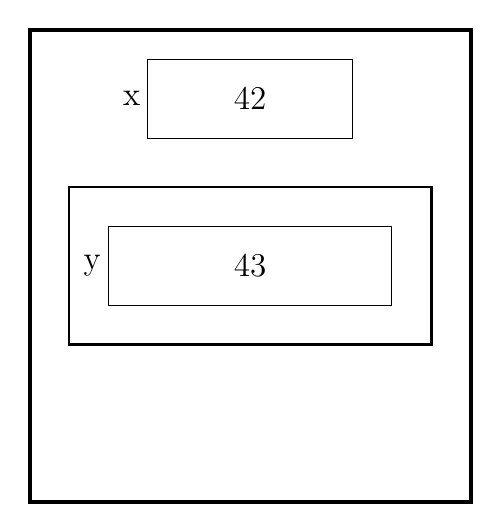
\begin{tikzpicture}
    \node[draw,text width=5cm,minimum height=6cm,minimum width=3cm, line width=0.05cm, inner sep=0.3cm] (a) at (-3.8,-2) {};
    \node[draw,text width=3cm, minimum height=1cm, line width=0.01cm, inner sep=0.3cm] (b) at (a.center) {};
    \node (fortythree) at (b.center) {\large{43}};
    \node[draw,text width=4cm, minimum height=2cm, line width=0.035cm, inner sep=0.3cm] (c) at (b.center) {};
    \node[draw, yshift=-9mm, text width=2cm, minimum height=1cm, line width=0.01cm, inner sep=0.3cm] (d) at (a.north) {};
    \node[xshift=-2mm] (ymemnode) at (b.west) {\large{y}};
    \node[xshift=-2mm] (xmemnode) at (d.west) {\large{x}};
    \node (fortytwo) at (d.center) {\large{42}};
    
    %% \draw [dashed, thick, ->] (ivar.north) to (b.center);
    %% \draw [dashed, thick, ->] (forloop.south) to (b.north);
    
\end{tikzpicture}
}

\begin{consolethree}[escapeinside=||]
#include <iostream>

int main()
{    
     int x = 0;
     std::cin >> x;
     
     if (x == 42)
     {   
         std::cout << "here we go ..." << std::endl;
         int y = x + 1;
         std::cout << "y: " << y << std::endl;
     }
     std::cout << "y: " << y << std::endl;

     return 0;
}
\end{consolethree}

\begin{consolethree}[escapeinside=||]
#include <iostream>

int main()
{    
     int x = 0;
     std::cin >> x;

     if (x == 42)
     {   
         std::cout << "here we go ..." <<
         std::endl;
         int y = x + 1;
         std::cout << "y: " << y << std::endl;
     }
     std::cout << "y: " << y << std::endl;

     return 0;
}
\end{consolethree}

%% As you can see, immediately on exiting the \texttt{if} statement, the \EMPHASIZE{variable in the body of the }\texttt{\EMPHASIZE{if}}\EMPHASIZE{statement is destroyed}.

%% Of course \texttt{x} was created in the \texttt{main()} block. So \texttt{x} is not destroyed.

%% This is one of the reasons why proper indentation is so important. Not only does it help you read the logic of your code, it tells you when variables are destroyed.

%% \newpage\EMPHASIZE{\texttt{for}-loops and \texttt{while}-loops}

%% You should think of the \emph{for}-loop as having a block and the body
%% of the for-loop as having an inner block.

%% \begin{console}
%% \#include < iostream>

%% int main()

%% \{

%% int x = 42, p = 1;

%% for (int i = 1; i <= x; ++i)

%% \{

%% int y = i * i;

%% \vtop{\hbox{\strut  p *= y;}\hbox{\strut  \}}}

%% std::cout << p << std::endl;

%% \vtop{\hbox{\strut  return 0;}\hbox{\strut \}}} \\
%% \end{console}

%% As we enter the \emph{for}-loop, we get a block of memory for the
%% \emph{for}-loop. Variable \emph{i} in the \emph{for}-loop resides in
%% this block.

%% \begin{console}
%% \#include < iostream>

%% int main()

%% \{

%% int x = 42, p = 1;

%% for (int i = 1; i <= x; ++i)

%% \{

%% int y = i * i;

%% \vtop{\hbox{\strut  p *= y;}\hbox{\strut  \}}}

%% std::cout << p << std::endl;

%% \vtop{\hbox{\strut  return 0;}\hbox{\strut \}}} \\
%% \end{console}

%% When we step into the body of the \emph{for}-loop, we have
%% \emph{\textbf{another}} block. Variable \emph{y} is created in this
%% inner block:

%% \begin{console}
%% \#include < iostream>

%% int main()

%% \{

%% int x = 42, p = 1;

%% for (int i = 1; i <= x; ++i)

%% \{

%% int y = i * i;

%% \vtop{\hbox{\strut  p *= y;}\hbox{\strut  \}}}

%% std::cout << p << std::endl;

%% \vtop{\hbox{\strut  return 0;}\hbox{\strut \}}} \\
%% \end{console}

%% When the last statement of the body of the \emph{for}-loop is executed,
%% we exit the body and variable \emph{y} is destroyed:

%% \begin{console}
%% \#include < iostream>

%% int main()

%% \{

%% int x = 42, p = 1;

%% for (int i = 1; i <= x; ++i)

%% \{

%% int y = i * i;

%% \vtop{\hbox{\strut  p *= y;}\hbox{\strut  \}}}

%% std::cout << p << std::endl;

%% \vtop{\hbox{\strut  return 0;}\hbox{\strut \}}} \\
%% \end{console}

%% Of course when we enter the body of the \emph{for}-loop the second time
%% (when \emph{i} = 2), variable \emph{y} is created again.

%% Get it?

%% And when we exit the \emph{for}-loop altogether, variable \emph{i} is
%% destroyed because it is created in the \emph{for}-loop:

%% \begin{console}
%% \#include < iostream>

%% int main()

%% \{

%% int x = 42, p = 1;

%% for (int i = 1; i <= x; ++i)

%% \{

%% int y = i * i;

%% \vtop{\hbox{\strut  p *= y;}\hbox{\strut  \}}}

%% std::cout << p << std::endl;

%% \vtop{\hbox{\strut  return 0;}\hbox{\strut \}}} \\
%% \end{console}

%% Note that variable \emph{x} and \emph{p} are still in scope; they are
%% not destroyed.

%% What about the \emph{while}-loop? The idea is similar: The
%% \emph{while}-loop has it' s memory and the body of the
%% \emph{while}-loop has an inner block.

%% \begin{console}
%% \#include < iostream>

%% int main()

%% \{

%% ...

%% int x = 42;

%% while (...)

%% \{

%% int y = 24;

%% \vtop{\hbox{\strut  ...}\hbox{\strut  \}}}

%% \vtop{\hbox{\strut  ...}\hbox{\strut \}}} \\
%% \end{console}

%% So remember this: each loop has it' s own memory for
%% variables and the body of the loop itself has its own memory.

%% \textbf{Exercise.} What is the problem? Fix it!

%% \begin{console}

%% std::cout << "Compute product of squares.";



%% std::cout << "Enter 0 to stop.\textbackslash n";






%% int prod = 1;



%% int x;



%% std::cin >> x;



%% while (x != 0)



%% \{



%% int square = x * x;



%% prod = prod * square;



%% std::cout << "Product:" << prod
%% << "\textbackslash n";



%% std::cin >> x;



%% \}






%% std::cout << "\textbackslash nProduct:"
%% << prod << std::endl;



%% std::cout << "Last square: " <<
%% square



%% << std::endl;
%%  \\
%% \end{console}

%% If you need \textbf{several} temporary variables in a \emph{for}-loop
%% you can do this:

%% \begin{console}
%% for (\textbf{int i = 0, s = 5, t = 100}; i < 10; i++)

%% \{

%% \vtop{\hbox{\strut  ...}\hbox{\strut \}}} \\
%% \end{console}

%% For instance if you want to print the running partial sums of summing 1
%% to 100 you can do this:

%% \begin{console}
%% for (int i = 0, s = 0; i < 10; i++)

%% \{

%% s += i;

%% \vtop{\hbox{\strut  std::cout << i
%% << ' '
%% << s <<
%% '\textbackslash n';}\hbox{\strut \}}} \\
%% \end{console}

%% Of course note that in this case \emph{s} is local to the
%% \emph{for}-loop and hence goes out of scope when the \emph{for}-loop is
%% done, i.e., it cannot be referenced outside the \emph{for}-loop:

%% \begin{console}
%% for (int i = 0, s = 0; i < 10; i++)

%% \{

%% s += i;

%% \vtop{\hbox{\strut  std::cout << i
%% << ' ' s
%% <<
%% '\textbackslash n';}\hbox{\strut \}}}

%% std::cout << s <<
%% '\textbackslash n'; //
%% BADDDDDDDDDDDDD!!!! \\
%% \end{console}

%% \textbf{Exercise.} Can you also create variables in the header of an
%% \emph{if} statement? Can this work:

%% \begin{console}
%% int i = 0;

%% if (int x = i * i < 10)

%% \{

%% ... do something with i and x ...

%% \}

%% ... do not use x!!! ... \\
%% \end{console}

%% Variables with the same name

%% Pay attention!!! This is something new!!!

%% You can actually create variables with the same name ... provided they
%% are either declared in non-overlapping blocks or one is defined in an
%% inner block.

%% Here' s the case where names are created in
%% \textbf{disjoint blocks}:

%% \begin{console}
%% ...

%% for (int i = 0; i < 10; ++i)

%% \{

%% int x, y, z;

%% ...

%% \}

%% for (int i = 0; i < 100; ++i)

%% \{

%% ...

%% int y;

%% \}

%% ... \\
%% \end{console}

%% Do you see why there won' t be conflicts or confusion to
%% C++?

%% Here' s the case where two names are created in
%% \textbf{nested blocks}:

%% \begin{console}
%% int x = 0, y = 0;

%% std::cin >> x >> y;

%% if (x == 0)

%% \{

%% int a = 5;

%% std::cout << a << std::endl;

%% if (y == 1)

%% \{

%% int a = 6;

%% std::cout << a << std::endl;

%% \}

%% \} \\
%% \end{console}

%% YIKES!!!

%% Note that the first print statement is not ambiguous. (Why?)

%% But what about the second? Which \emph{a} is used in the second print
%% statement???... go to next section to find out ...

%% WARNING: Although technically you can do the above (i.e. have two
%% variables with the same name nest within blocks, it makes the code hard
%% to read. Not only that, some languages do not allow this at all.
%% Therefore you should \textbf{AVOID DECLARING VARIABLES WITH THE SAME
%% NAME IN NESTED BLOCKS}. The only \textbf{exception} is a temporary
%% (scratch) variable for instance like the counter variable of a
%% \emph{for}-loop

%% \begin{console}
%% for (int i = 0; i < 100; i++)

%% \{

%% ...

%% for (int i = -10; i < 10; i++)

%% \{

%% ...

%% \vtop{\hbox{\strut  \}}\hbox{\strut  ...}}

%% \emph{\}}  \\
%% \end{console}

%% and only when the logic is easy to understand. But even then, you might
%% still be shooting yourself in your foot later if you need to change the
%% logic of your code.

%% How does C++ search for a variable?

%% In looking for a variable C++ will always start from the block where the
%% execution occurs. If the variable cannot be found, C++ will look for
%% that variable in the nearest outer enclosing block.

%% Here' s a simple example:

%% \begin{console}

%% \#include < iostream>



%% int main()



%% \{



%% int i = 5;






%% if ( i > 0 )



%% \{



%% int j = 6;



%% std::cout << i;



%% \}






%% return 0;



%% \}
%%  \\
%% \end{console}

%% Of course C++ might need to search in several enclosing blocks before
%% it' s found.




%% \begin{console}
%% \#include < iostream>

%% int main()

%% \{

%% int i = 5;

%% while (i > 0)

%% \{

%% int j = 6;

%% for (int k = 0; k < j; ++k)

%% \{

%% \vtop{\hbox{\strut  std::cout << i;}\hbox{\strut  \}}}

%% -\/-i;

%% \}

%% \} \\
%% \end{console}

%% \textbf{Exercise.} Now look at the example from the previous section.
%% Why is

%% C++ not confused?

%% \begin{console}
%% int x = 0, y = 0;

%% std::cin >> x >> y;

%% if (x == 0)

%% \{

%% int a = 5;

%% std::cout << a << std::endl;

%% if (y == 1)

%% \{

%% int a = 6;

%% std::cout << a << std::endl;

%% \}

%% \} \\
%% \end{console}

%% In this case when the variable \emph{a} in the inner if-statement is
%% created, we say that the innermost \emph{a} \textbf{hides} the outer
%% \emph{a}.

%% \textbf{Exercise.} What is the output? (Or is there an error?)

%% \begin{console}
%% int x = 0, y = 1;

%% if (x == 0)

%% \{

%% int a = 5;

%% if (y == 1)

%% \{

%% std::cout << a << std::endl;

%% int a = 6;

%% std::cout << a << std::endl;

%% \}

%% \} \\
%% \end{console}

%% \textbf{Exercise.} What is the output? (Or is there an error?)

%% \begin{console}
%% int x = 0, y = 1;

%% for (int x = 5; x < 10; x++)

%% \{

%% std::cout << x << '
%% ' << y <<
%% std::endl;

%% int y = 5;

%% while (y > 0)

%% \{

%% int x = y + 1;

%% std::cout << x << '
%% ' << y <<
%% std::endl;

%% \vtop{\hbox{\strut  y++;}\hbox{\strut  \}}}

%% std::cout << x << '
%% ' << y <<
%% std::endl;

%% \} \\
%% \end{console}

%% \textbf{Exercise.} What is the output? (Or is there an error?)

%% \begin{console}[]{@l@}
%% \toprule\noalign
%%  \\
%% \midrule\noalign
%% \endhead
%% \bottomrule\noalign
%% \endlastfoot
%% \vtop{\hbox{\strut int i = 5, j = 6;}\hbox{\strut std::cout
%% << i << '
%% ' << j <<
%% std::endl;}\hbox{\strut for (int i = 0; i < 3;
%% i++)}\hbox{\strut \\hbox{\strut  std::cout << i
%% << ' '
%% << j << std::endl;}\hbox{\strut  if
%% (i < j)}\hbox{\strut  \\hbox{\strut  std::cout
%% << i << '
%% ' << j <<
%% std::endl;}\hbox{\strut  int i = 24;}\hbox{\strut  std::cout
%% << i << '
%% ' << j <<
%% std::endl;}\hbox{\strut  \}}\hbox{\strut  else}\hbox{\strut 
%% \\hbox{\strut  std::cout << i <<
%% ' ' << j
%% << std::endl;}\hbox{\strut  int j = 42;}\hbox{\strut 
%% std::cout << i << '
%% ' << j <<
%% std::endl;}\hbox{\strut  \}}\hbox{\strut  std::cout <<
%% i << ' '
%% << j <<
%% std::endl;}\hbox{\strut \}}\hbox{\strut std::cout << i
%% << ' '
%% << j << std::endl;}} \\
%% \end{console}

%% \textbf{Exercise.} What is the output? (Or is there an error?)

%% \begin{console}
%% \vtop{\hbox{\strut int i = 5, j = 6;}\hbox{\strut std::cout
%% << i << '
%% ' << j <<
%% std::endl;}\hbox{\strut for (int i = 0; i < 3;
%% i++)}\hbox{\strut \}

%% \vtop{\hbox{\strut  int i = 8;}\hbox{\strut  std::cout
%% << i << '
%% ' << j <<
%% std::endl;}\hbox{\strut  if (i < j)}\hbox{\strut 
%% \\hbox{\strut  std::cout << i <<
%% ' ' << j
%% << std::endl;}\hbox{\strut  int i = 24;}\hbox{\strut 
%% std::cout << i << '
%% ' << j <<
%% std::endl;}\hbox{\strut  \}}\hbox{\strut  else}\hbox{\strut 
%% \\hbox{\strut  std::cout << i <<
%% ' ' << j
%% << std::endl;}\hbox{\strut  int j = 42;}\hbox{\strut 
%% std::cout << i << '
%% ' << j <<
%% std::endl;}\hbox{\strut  \}}\hbox{\strut  std::cout <<
%% i << ' '
%% << j << std::endl;}}

%% \vtop{\hbox{\strut  int i = 9;}\hbox{\strut \}}\hbox{\strut std::cout
%% << i << '
%% ' << j <<
%% std::endl;}} \\
%% \end{console}

%% Principle of minimal scope


%% Here' s the principle of minimal scope:






%% Keep the scope of variables



%% as small as possible.






%% (The above is suppose to blink).






%% For instance this is NOT GOOD:


%% \begin{console}
%% // compute the factorial of n

%% int i = 0;

%% int prod = 1;

%% int n = 0;

%% std::cin >> n;

%% for (i = 1; i <= n; i++)

%% \{

%% \vtop{\hbox{\strut  prod *= i;}\hbox{\strut \}}}

%% std::cout << prod << std::endl; \\
%% \end{console}





%% This is BETTER


%% \begin{console}
%% // compute the factorial of n

%% int prod = 1;

%% int n = 0;

%% std::cin >> n;

%% for (int i = 1; i <= n; i++)

%% \{

%% \vtop{\hbox{\strut  prod *= i;}\hbox{\strut \}}}

%% std::cout << prod << std::endl; \\
%% \end{console}








%% \textbf{Exercise.} What' s the difference?









%% Why? Frequently when you' re solving a problem (not just
%% a programming problem), you go through a sequence of steps of
%% computation or transformation on the data. Each step usually requires
%% some input data to modify something (such as a variable) or to perform a
%% task (such as printing something to the screen in a game).






%% For our program above you should be able to see these steps:




















































































%% A well-written program will always try to minimize the inputs and
%% outputs (or change) within a step such as this:

%% .

%% Why? Because the more stuff you have in a step the more complex it will
%% be. That means that the code is harder to read, debug, and maintain for
%% future change. In the real world, software engineers write new code and
%% maintain code base (maintain = correct, add and delete). Now look at
%% this:
%% /
%% What variables are involved in this step? Don' t think
%% about the internals of this chunk of code. Think of the code as a black
%% box. You need n (that' s the input) and you want to
%% compute the factorial of n (that' s the output) and you
%% want to put that value into prod (that' s the
%% transformation).






%% So two variables take part in this step.

%% Now look at the code from the first program (the part in bold):

%% \begin{console}
%% // compute the factorial of n

%% int i = 0;

%% int prod = 1;

%% int n = 0;

%% std::cin >> n;

%% for (i = 1; i <= n; i++)
%% {

%%  prod *= i;

%% }

%% std::cout << prod << std::endl; 
%% \end{console}

%% You see clearly that besides ``sending in'' variables \emph{n} and \emph{prod} to this step, \emph{\textbf{you also ``send in'' variable }\textbf{i}}.

%% Now look at the improved version:

%% \begin{console}
%% // compute the factorial of n

%% int prod = 1;

%% int n = 0;

%% std::cin >> n;

%% for (int i = 1; i <= n; i++)
%% {

%%   prod *= i;

%% }

%% std::cout << prod << std::endl; \\
%% \end{console}

%% Variable \emph{i} is internal to the step that computes the factorial of
%% \emph{n} and stores it in \emph{prod}. Outside the code that computes
%% and stores the factorial of \emph{n} in \emph{prod}, variable \emph{i}
%% does not exist.

%% Get it?

%% This also prevent ``side effects'' in code. (I've already mentioned this.) If a variable has a large scope, and you modify it in some place, it might have unexpected effects. Here's something similar to a previous example -- it's important enough to repeat!!! For instance suppose work in a team and you're given this code segment:


%% \begin{console}
%% ...

%% int i = 42;

%% ...

%% for (; i < 100; i++)
%% {

%%   ...

%% }

%% .... 
%% \end{console}

%% where you expect the \emph{for}-loop to run from \emph{i} = 42 to
%% \emph{i} = 99. One of your colleagues might see the variable \emph{i}
%% and add some code like so:

%% \begin{console}
%% ...

%% int i = 42;

%% ...

%% for (i = 1000; i > 0; --i)

%% {

%% ...

%% }

%% ...

%% for (; i < 100; i++)

%% {

%%  ...

%% }

%% .... 
%% \end{console}

%% So guess what? When you use \emph{i}, the initial value for you is now 0 and not 42 and your program doesn't work anymore. Tough. What's worse is when you try to debug, you might not even see it because you kept saying to yourself ``But, but, but ... I didn't change anything ever since it was working!!! ... and my code looks the same as before!!!''

%% This is one of the most important reasons why we also try to restrict the scope of a variable. If it's meant to be a ``scratch'' variable, then create it in such a way that it gets destroy ASAP.

%% As you can see from the example, one way to minimize scopes is to declare only when you need to and in the \textbf{innermost block} whenever possible. For our example, we declare \emph{i} within the for-loop block.

%% \textbf{NOTE: }Some people declare all variables at the beginning of a function. That's because \emph{\textbf{some}} programming languages specify that \emph{\textbf{all}} declaration statements must come before other types of statements.
%% That's not the case for C++ or other modern programming languages.

%% Now let's go back to that program again.
%% There's one other spot where you can minimize the scope
%% of a variable.

%% \begin{console}
%% // compute the factorial of n

%% int prod = 1;

%% int n = 0;

%% std::cin >> n;

%% for (int i = 1; i <= n; i++)

%% {

%% prod *= i;
%% }

%% std::cout << prod << std::endl; \\
%% \end{console}

%% Note that \emph{prod} is not used until the \emph{for}-loop. So you can
%% write this:

%% \begin{console}
%% // compute the factorial of n

%% int n = 0;

%% std::cin >> n;

%% int prod = 1;

%% for (int i = 1; i <= n; i++)

%% {

%% prod *= i;

%% std::cout << prod << std::endl;
%% }
%% \end{console}

%% This however is \textbf{not as crucial} as the previous change because
%% \emph{prod} is not destroyed. Furthermore \emph{prod} is part of the
%% larger goal of computing the factorial. Hence it' s OK to
%% declare \emph{prod} early so that readers of your code can see it early,
%% especially if you mention \emph{prod} in your comments like this:

%% \begin{console}
%% // compute the factorial of n and store it in prod

%% int n = 0;

%% int prod = 1;

%% std::cin >> n;

%% for (int i = 0; i <= n; i++)

%% {

%%  prod *= i;

%% std::cout << prod << std::endl;
%% }
%% \end{console}

%% See that?

%% \textbf{Exercise.} Rewrite the following program so that variables have
%% minimal scopes.

%% \begin{console}
%% #include <iostream>

%% int main()
%% {

%% int answer, i, first, last, sum, term;

%% std::cout << "Find sum? (1 -- yes or 0 - no) ";

%% std::cin >> answer;

%% if (answer == 1)

%% {

%% std::cout << "First int:";

%% std::cin >> first;

%% std::cout << "Last int:"

%% std::cin >> last;

%% sum = 0;

%% for (i = first; i <= last; ++i)

%% {

%% term = i * i * i * i;

%% sum += term;
%% }

%% std::cout << "Sum:" << sum
%% << std::endl;
%% }

%% return 0;

%% }
%% \end{console}





%% \begin{ex} The following program computes the sum

%% (1/1) + (1/1)(1/2) + (1/1)(1/2)(1/3) + (1/1)(1/2)(1/3)(1/4) + ...
    
%% (that's in mathematical notation and not C++ notation)
%% where the number of terms is specified by the user. Verify by hand that
%% it does not work correctly. Explain why and correct the program; there
%% are several problems.


%% \begin{console}
%% int n = 0, i = 0, j = 0, term = 0, sum = 0;

%% std::cin >> n;

%% for (i = 1; i <= n; ++i)

%% {

%% // Compute i-th term, i.e. 1/1*...*1/i

%% for (j = 0; j < i; ++j)

%% {

%% term *= 1.0 / j;

%% // Accumulate term into sum by addition

%%   sum += term;

%% std::cout << sum << std::endl; \\
%% \end{console}

%% \newpage\EMHPASIZE{Summary}
%% The scope of a variable is where the variable can be accessed. This is
%% from the declaration of the variable to the end of the block where it is
%% declared.
%% ...
%% {
%% ...
%% double i = 0.0;
%% ...
%% }

%% ...

%% If a variable name is used in two declarations, then the two blocks
%% where they are declared do not overlap or one is nested within the
%% other.

%% If the program tries to access a variable and it' s not
%% found in the current block, then the program will look for the variable
%% in the \emph{\textbf{nearest}} outer block.

%% The \emph{for}-loop and \emph{while}-loop create a block and their
%% bodies create a block within the loop's block.
